% =====================================================================
\chapter{Estadística descriptiva}
\label{tema:1}
% =====================================================================

Antes de construir modelos conviene mirar los datos: resumirlos con unos pocos números y dibujarlos. Este tema presenta las medidas de centralización (media, mediana), de posición (cuantiles y cuartiles), de dispersión (rango, recorrido intercuartílico, varianza y desviación típica), las representaciones gráficas básicas (histograma y diagrama de caja) y las medidas de relación entre dos variables (covarianza y correlación). Se sigue el capítulo~2 de \emph{Introductory Statistics} de OpenStax~\cite{openstax} (§2.2 a §2.7), el capítulo~10 de Rice~\cite{rice}, «Summarizing Data», y, para la covarianza y la correlación, la lectura~7b del curso 18.05 del MIT~\cite{mit1805} y la §7.3 de Blitzstein y Hwang~\cite{bh}.

\section{Datos, población y muestra}

\begin{definicion}[Población, muestra y variable]\label{def:t1-poblacion}
La \emph{población} es el conjunto de todos los individuos u objetos sobre los que se quiere obtener información; una \emph{muestra} es un subconjunto de la población que efectivamente se observa. Una \emph{variable} es una característica que se mide en cada individuo. La variable es \emph{cuantitativa} si toma valores numéricos con los que tiene sentido operar (discreta si toma valores aislados, como un número de errores; continua si puede tomar cualquier valor de un intervalo, como un tiempo) y \emph{cualitativa} o \emph{categórica} si toma valores en un conjunto de categorías.
\end{definicion}

Un conjunto de datos cuantitativos es una lista $x_1,\dots,x_n$ de números reales, donde $n$ es el \emph{tamaño} de la muestra. Los mismos datos ordenados de menor a mayor se escriben $x_{(1)}\le x_{(2)}\le\dots\le x_{(n)}$; $x_{(1)}$ es el mínimo y $x_{(n)}$, el máximo. En este tema los datos son números fijos y las definiciones son puramente descriptivas; a partir del \cref{tema:2} se interpretarán como valores observados de variables aleatorias.

\begin{ejemplo}[Datos de referencia]\label{ej:t1-tokens}
Se miden las longitudes, en tokens, de ocho respuestas de un modelo de lenguaje:
\[
12,\quad 15,\quad 11,\quad 18,\quad 14,\quad 40,\quad 13,\quad 16.
\]
Ordenados: $11,12,13,14,15,16,18,40$. Este conjunto se usará como ejemplo a lo largo del tema; el valor $40$ es claramente mayor que los demás.
\end{ejemplo}

\section{Medidas de centralización}

\begin{definicion}[Media, mediana y moda]\label{def:t1-centro}
Sean $x_1,\dots,x_n$ datos reales.
\begin{enumerate}
  \item La \emph{media} (aritmética) es $\displaystyle\xbar=\frac1n\sum_{i=1}^{n}x_i$.
  \item La \emph{mediana} es el valor central de los datos ordenados: $x_{((n+1)/2)}$ si $n$ es impar, y $\tfrac12\bigl(x_{(n/2)}+x_{(n/2+1)}\bigr)$ si $n$ es par.
  \item La \emph{moda} es el valor que aparece con mayor frecuencia (puede no ser única).
\end{enumerate}
\end{definicion}

\begin{ejemplo}\label{ej:t1-media-mediana}
En el \cref{ej:t1-tokens}, $\sum x_i=139$ y $\xbar=139/8=17{,}375$. Como $n=8$ es par, la mediana es la media de los valores cuarto y quinto ordenados: $(14+15)/2=14{,}5$. Si se elimina el valor $40$, la media pasa a $99/7\approx 14{,}14$ y la mediana a $14$: la media se ha desplazado más de tres unidades y la mediana, media unidad.
\end{ejemplo}

El ejemplo ilustra que la media es \emph{sensible a los valores atípicos} y la mediana es \emph{robusta}. Cuando la distribución de los datos es asimétrica con cola larga a la derecha (como las longitudes de respuesta, los tiempos o los ingresos), la media suele ser mayor que la mediana~\cite[§2.6]{openstax}. Las dos medidas tienen una caracterización variacional que explica ese comportamiento.

\begin{proposicion}[Propiedades extremales de la media y la mediana]\label{prop:t1-extremal}
Sean $x_1,\dots,x_n$ datos reales.
\begin{enumerate}
  \item $\sum_{i=1}^{n}(x_i-\xbar)=0$.
  \item Para todo $a\in\R$, $\displaystyle\sum_{i=1}^{n}(x_i-a)^{2}=\sum_{i=1}^{n}(x_i-\xbar)^{2}+n(\xbar-a)^{2}$. En consecuencia, la función $a\mapsto\sum_i(x_i-a)^{2}$ alcanza su mínimo únicamente en $a=\xbar$.
  \item La función $a\mapsto\sum_i\abs{x_i-a}$ alcanza su mínimo en la mediana.
\end{enumerate}
\end{proposicion}

\begin{proof}
(i) $\sum_i(x_i-\xbar)=\sum_i x_i-n\xbar=n\xbar-n\xbar=0$.

(ii) Se escribe $x_i-a=(x_i-\xbar)+(\xbar-a)$ y se desarrolla el cuadrado:
\[
\sum_i(x_i-a)^{2}=\sum_i(x_i-\xbar)^{2}+2(\xbar-a)\sum_i(x_i-\xbar)+n(\xbar-a)^{2}.
\]
El término central es nulo por (i). El último sumando es no negativo y solo se anula si $a=\xbar$.

(iii) Se demuestra en el \cref{eje:t1-mediana-min}.
\end{proof}

\section{Medidas de posición: cuantiles y diagrama de caja}

La mediana divide los datos ordenados en dos mitades. Los cuartiles los dividen en cuatro partes. Hay varias convenciones para calcularlos que dan resultados ligeramente distintos con pocos datos (los programas estadísticos suelen interpolar); en este módulo se usa la siguiente, que es la de~\cite[§2.3]{openstax} y la habitual en el cálculo a mano.

\begin{definicion}[Cuartiles y recorrido intercuartílico]\label{def:t1-cuartiles}
Sean $x_{(1)}\le\dots\le x_{(n)}$ los datos ordenados. La \emph{mitad inferior} está formada por los $\lfloor n/2\rfloor$ primeros datos y la \emph{mitad superior}, por los $\lfloor n/2\rfloor$ últimos (si $n$ es impar, la mediana no pertenece a ninguna de las dos). El \emph{primer cuartil} $Q_1$ es la mediana de la mitad inferior; el \emph{segundo cuartil} $Q_2$ es la mediana; el \emph{tercer cuartil} $Q_3$ es la mediana de la mitad superior. El \emph{recorrido intercuartílico} es $\RIC=Q_3-Q_1$ y el \emph{rango} es $x_{(n)}-x_{(1)}$.
\end{definicion}

Más en general, el \emph{cuantil} de orden $q\in(0,1)$ (o \emph{percentil} $100q$) es un valor que deja a su izquierda aproximadamente una fracción $q$ de los datos; $Q_1$, $Q_2$ y $Q_3$ son los cuantiles de órdenes $0{,}25$, $0{,}5$ y $0{,}75$.

\begin{definicion}[Resumen de cinco números y diagrama de caja]\label{def:t1-caja}
El \emph{resumen de cinco números} es $(x_{(1)},Q_1,Q_2,Q_3,x_{(n)})$. Un dato se considera \emph{atípico} (criterio de Tukey) si está fuera del intervalo
\[
\bigl[\,Q_1-1{,}5\,\RIC,\;Q_3+1{,}5\,\RIC\,\bigr],
\]
cuyos extremos se llaman \emph{vallas}. El \emph{diagrama de caja} dibuja una caja de $Q_1$ a $Q_3$ con una línea en la mediana y dos «bigotes» que llegan hasta el dato más extremo no atípico de cada lado; los atípicos se marcan por separado~\cite[§2.4]{openstax}.
\end{definicion}

\begin{ejemplo}\label{ej:t1-cuartiles}
En el \cref{ej:t1-tokens}, $n=8$, la mitad inferior es $11,12,13,14$ y la superior $15,16,18,40$. Entonces $Q_1=(12+13)/2=12{,}5$, $Q_2=14{,}5$, $Q_3=(16+18)/2=17$ y $\RIC=4{,}5$. Las vallas son $12{,}5-6{,}75=5{,}75$ y $17+6{,}75=23{,}75$, de modo que $40$ es atípico. El bigote superior llega hasta $18$.
\end{ejemplo}

\begin{figure}[ht]
\centering
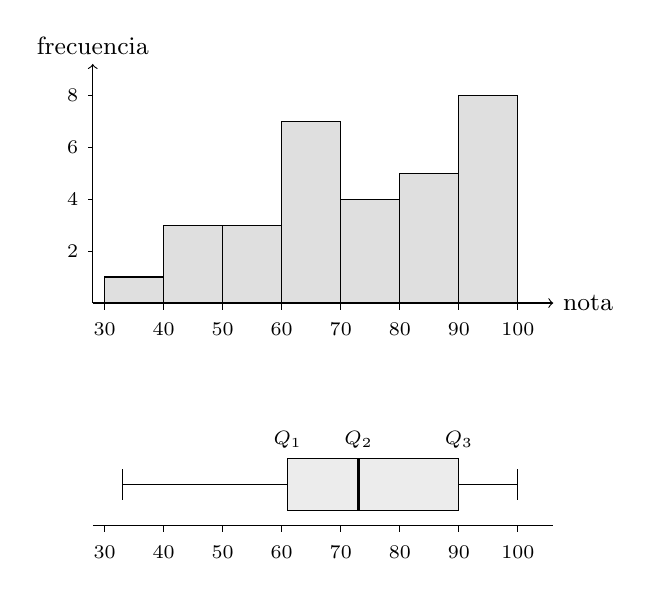
\begin{tikzpicture}[x=0.075cm,y=0.33cm]
  % Histograma
  \foreach \a/\h in {30/1,40/3,50/3,60/7,70/4,80/5,90/8}{
    \draw[fill=gray!25] (\a,0) rectangle (\a+10,\h);
  }
  \draw[->] (28,0) -- (106,0) node[right]{\small nota};
  \draw[->] (28,0) -- (28,9.2) node[above]{\small frecuencia};
  \foreach \a in {30,40,...,100}{\draw (\a,0) -- (\a,-0.25) node[below,text height=1.4ex,text depth=0.2ex]{\scriptsize\a};}
  \foreach \h in {2,4,6,8}{\draw (28,\h) -- (27.2,\h) node[left]{\scriptsize\h};}
  % Diagrama de caja
  \begin{scope}[yshift=-2.3cm]
    \draw (33,0) -- (61,0); \draw (90,0) -- (100,0);
    \draw (33,-0.6) -- (33,0.6); \draw (100,-0.6) -- (100,0.6);
    \draw[fill=gray!15] (61,-1) rectangle (90,1);
    \draw[thick] (73,-1) -- (73,1);
    \foreach \a in {30,40,...,100}{\draw (\a,-1.6) -- (\a,-1.85) node[below,text height=1.4ex,text depth=0.2ex]{\scriptsize\a};}
    \draw (28,-1.6) -- (106,-1.6);
    \node[above] at (61,1) {\scriptsize $Q_1$};
    \node[above] at (73,1) {\scriptsize $Q_2$};
    \node[above] at (90,1) {\scriptsize $Q_3$};
  \end{scope}
\end{tikzpicture}
\caption{Histograma (clases de amplitud 10) y diagrama de caja de las 31 notas de examen del ejemplo~2.33 de~\cite{openstax}: mínimo 33, $Q_1=61$, mediana 73, $Q_3=90$, máximo 100. La cola izquierda más larga se aprecia en ambos gráficos.}\label{fig:t1-hist-caja}
\end{figure}

\begin{definicion}[Histograma]\label{def:t1-histograma}
Se divide un intervalo que contiene los datos en \emph{clases} contiguas $[a_0,a_1),[a_1,a_2),\dots,[a_{k-1},a_k]$ y se cuenta la \emph{frecuencia absoluta} $f_j$ de datos en cada clase. El \emph{histograma} dibuja sobre cada clase un rectángulo de altura proporcional a $f_j$ (si las clases tienen igual amplitud) o a $f_j/(a_j-a_{j-1})$ (si no la tienen, de modo que el \emph{área} sea proporcional a la frecuencia). La \emph{frecuencia relativa} es $f_j/n$.
\end{definicion}

El histograma muestra la forma de la distribución (simetría, asimetría, número de modas), mientras que el diagrama de caja resume la posición y la dispersión y señala los atípicos; la \cref{fig:t1-hist-caja} muestra ambos para un mismo conjunto de datos.

\section{Medidas de dispersión}

\begin{definicion}[Varianza y desviación típica muestrales]\label{def:t1-varianza}
La \emph{varianza muestral} de $x_1,\dots,x_n$ ($n\ge 2$) es
\[
s^{2}=\frac{1}{n-1}\sum_{i=1}^{n}(x_i-\xbar)^{2},
\]
y la \emph{desviación típica muestral} es $s=\sqrt{s^{2}}$. La cantidad $\sum_i(x_i-\xbar)^{2}$ se llama \emph{suma de cuadrados} de los datos.
\end{definicion}

\begin{observacion}[¿Por qué $n-1$?]\label{obs:t1-n-1}
El denominador $n-1$ en lugar de $n$ tiene dos justificaciones. La primera es algebraica: las $n$ desviaciones $x_i-\xbar$ suman cero (\cref{prop:t1-extremal}), de modo que solo $n-1$ de ellas pueden elegirse libremente; se dice que la suma de cuadrados tiene $n-1$ \emph{grados de libertad}. La segunda es estadística: si los datos son una muestra aleatoria de una población con varianza $\sigma^{2}$, la versión con $n-1$ acierta «en promedio», es decir, es un estimador insesgado de $\sigma^{2}$, mientras que la versión con $n$ la subestima sistemáticamente. Esto se demuestra en el \cref{tema:2} (\cref{teo:t2-s2}). Con denominador $n$ se obtiene la \emph{varianza poblacional} de los propios datos, $\frac1n\sum_i(x_i-\xbar)^{2}$, que es la que se usa cuando los datos \emph{son} toda la población o cuando se normaliza un vector, como en la normalización por capas de una red (módulo~11).
\end{observacion}

\begin{proposicion}[Fórmula de cálculo]\label{prop:t1-abreviada}
$\displaystyle\sum_{i=1}^{n}(x_i-\xbar)^{2}=\sum_{i=1}^{n}x_i^{2}-n\xbar^{2}$, y por tanto $s^{2}=\dfrac{\sum_i x_i^{2}-n\xbar^{2}}{n-1}$.
\end{proposicion}

\begin{proof}
Es el caso $a=0$ de la \cref{prop:t1-extremal}(ii): $\sum_i x_i^{2}=\sum_i(x_i-\xbar)^{2}+n\xbar^{2}$.
\end{proof}

\begin{ejemplo}\label{ej:t1-varianza}
En el \cref{ej:t1-tokens}, $\sum x_i^{2}=3035$ y $n\xbar^{2}=8\cdot 17{,}375^{2}=2415{,}125$. La suma de cuadrados es $3035-2415{,}125=619{,}875$, de donde $s^{2}=619{,}875/7\approx 88{,}55$ y $s\approx 9{,}41$. Sin el dato $40$ se obtiene $s\approx 2{,}41$: la desviación típica, como la media, es muy sensible a los atípicos, mientras que el $\RIC$ apenas cambia (de $4{,}5$ a $4$).
\end{ejemplo}

\begin{proposicion}[Cambios de escala y de origen]\label{prop:t1-lineal}
Si $y_i=ax_i+b$ con $a,b\in\R$, entonces $\ybar=a\xbar+b$, $s_y^{2}=a^{2}s_x^{2}$ y $s_y=\abs{a}\,s_x$. Si $a>0$, la mediana y los cuartiles se transforman igual que la media y $\RIC_y=a\,\RIC_x$.
\end{proposicion}

\begin{proof}
$\ybar=\frac1n\sum_i(ax_i+b)=a\xbar+b$. Entonces $y_i-\ybar=a(x_i-\xbar)$, y elevando al cuadrado y sumando, $\sum_i(y_i-\ybar)^{2}=a^{2}\sum_i(x_i-\xbar)^{2}$. Si $a>0$, la transformación conserva el orden, luego transforma los datos ordenados en datos ordenados y las medianas de cualquier subconjunto se transforman por $t\mapsto at+b$.
\end{proof}

\begin{definicion}[Tipificación]\label{def:t1-z}
Si $s>0$, la \emph{puntuación tipificada} (o puntuación $z$) del dato $x_i$ es $z_i=(x_i-\xbar)/s$. Por la \cref{prop:t1-lineal}, los datos tipificados tienen media $0$ y desviación típica $1$; $z_i$ mide a cuántas desviaciones típicas está $x_i$ de la media.
\end{definicion}

\section{Datos bivariantes: covarianza y correlación}

Cuando en cada individuo se miden dos variables se obtienen pares $(x_1,y_1),\dots,(x_n,y_n)$, que se representan en un \emph{diagrama de dispersión}.

\begin{definicion}[Covarianza y correlación muestrales]\label{def:t1-cov}
La \emph{covarianza muestral} y el \emph{coeficiente de correlación} (de Pearson) son
\[
s_{xy}=\frac{1}{n-1}\sum_{i=1}^{n}(x_i-\xbar)(y_i-\ybar),
\qquad
r=\frac{s_{xy}}{s_x\,s_y}=\frac{\sum_i(x_i-\xbar)(y_i-\ybar)}{\sqrt{\sum_i(x_i-\xbar)^{2}}\,\sqrt{\sum_i(y_i-\ybar)^{2}}},
\]
donde se supone $s_x,s_y>0$.
\end{definicion}

El signo de cada producto $(x_i-\xbar)(y_i-\ybar)$ es positivo cuando el punto está en el cuadrante superior derecho o inferior izquierdo respecto de $(\xbar,\ybar)$ y negativo en los otros dos; $s_{xy}>0$ indica que predominan los primeros, es decir, una tendencia creciente. La covarianza depende de las unidades; la correlación no (\cref{eje:t1-r-invariante}).

\begin{teorema}[Acotación de la correlación]\label{teo:t1-r}
Se cumple $-1\le r\le 1$. Además, $\abs{r}=1$ si y solo si existen $a\neq 0$ y $b$ tales que $y_i=ax_i+b$ para todo $i$, y entonces el signo de $r$ es el de $a$.
\end{teorema}

\begin{proof}
Sean $u_i=x_i-\xbar$ y $v_i=y_i-\ybar$, y $\mathbf u,\mathbf v\in\R^{n}$ los vectores correspondientes, ambos no nulos porque $s_x,s_y>0$. Entonces $r=\langle\mathbf u,\mathbf v\rangle/(\norm{\mathbf u}\norm{\mathbf v})$, y la desigualdad de Cauchy--Schwarz, $\abs{\langle\mathbf u,\mathbf v\rangle}\le\norm{\mathbf u}\norm{\mathbf v}$, da $\abs r\le 1$. La igualdad en Cauchy--Schwarz se da exactamente cuando $\mathbf v=a\mathbf u$ para algún $a\neq0$, es decir, $y_i-\ybar=a(x_i-\xbar)$ para todo $i$, que equivale a $y_i=ax_i+b$ con $b=\ybar-a\xbar$. En ese caso $\langle\mathbf u,\mathbf v\rangle=a\norm{\mathbf u}^{2}$ tiene el signo de $a$. Recíprocamente, si $y_i=ax_i+b$ entonces $v_i=au_i$ y $r=a\norm{\mathbf u}^{2}/(\norm{\mathbf u}\,\abs a\norm{\mathbf u})=a/\abs a=\pm1$.
\end{proof}

\begin{ejemplo}\label{ej:t1-r}
Para los pares $(1,2),(2,4),(3,5),(4,4),(5,5)$: $\xbar=3$, $\ybar=4$, $\sum(x_i-\xbar)^{2}=10$, $\sum(y_i-\ybar)^{2}=6$ y $\sum(x_i-\xbar)(y_i-\ybar)=(-2)(-2)+(-1)(0)+0\cdot1+1\cdot0+2\cdot1=6$. Entonces $s_{xy}=6/4=1{,}5$ y $r=6/\sqrt{60}\approx 0{,}775$: asociación lineal positiva moderadamente fuerte.
\end{ejemplo}

Los mismos conceptos existen para variables aleatorias. Si $(X,Y)$ es un vector aleatorio con varianzas finitas y positivas, su \emph{covarianza} y su \emph{correlación} son
\[
\Cov(X,Y)=\E\bigl[(X-\E X)(Y-\E Y)\bigr]=\E[XY]-\E[X]\E[Y],
\qquad
\Cor(X,Y)=\frac{\Cov(X,Y)}{\sqrt{\Var X\,\Var Y}},
\]
y también $\abs{\Cor(X,Y)}\le1$~\cite[§7.3]{bh}. Las fórmulas muestrales de la \cref{def:t1-cov} son las análogas con los datos (salvo el factor $n/(n-1)$, que se cancela en $r$).

\begin{observacion}[Errores frecuentes]\label{obs:t1-errores}
(a) Una correlación cercana a cero no significa que no haya relación, sino que no hay relación \emph{lineal}: para los puntos $(-2,4),(-1,1),(0,0),(1,1),(2,4)$, en los que $y=x^{2}$, se tiene $r=0$ (\cref{eje:t6-cuadratica}).
(b) Una correlación alta no implica causalidad (\cref{tema:6}).
(c) Calcular $s^{2}$ con denominador $n$ cuando se pide la varianza muestral, o confundir $s^{2}$ con $s$.
(d) Olvidar ordenar los datos antes de calcular la mediana o los cuartiles.
(e) Comparar medias de grupos muy asimétricos o con atípicos sin mirar también la mediana.
\end{observacion}

\begin{observacion}[Conexión con el curso]
La normalización por capas (\emph{LayerNorm}) del módulo~11 y de los Transformers del módulo~14 tipifica el vector de activaciones de cada token: le resta su media y lo divide por su desviación típica (con denominador $n$, como en la \cref{obs:t1-n-1}). Las tablas de resultados de los benchmarks de los módulos~22 y~23 son, en esencia, medias de variables $0$/$1$ (acierto o fallo), y los diagramas de caja son la forma habitual de mostrar la variabilidad entre semillas o entre ejecuciones de un mismo entrenamiento.
\end{observacion}

\begin{lecturas}
\item OpenStax~\cite{openstax}, cap.~2: §2.2 «Histograms, Frequency Polygons, and Time Series Graphs», §2.3 «Measures of the Location of the Data», §2.4 «Box Plots», §2.5 «Measures of the Center of the Data», §2.6 «Skewness and the Mean, Median, and Mode» y §2.7 «Measures of the Spread of the Data».
\item Rice~\cite{rice}, cap.~10 «Summarizing Data».
\item Orloff y Bloom~\cite{mit1805}, lectura~7b «Covariance and Correlation».
\item Blitzstein y Hwang~\cite{bh}, §7.3 «Covariance and correlation».
\end{lecturas}

\section*{Ejercicios del tema 1}
\addcontentsline{toc}{section}{Ejercicios del tema 1}

\begin{ejercicio}{1}{eje:t1-vf}
Indique si cada afirmación es verdadera o falsa y justifíquelo brevemente.
(a) Si se multiplica por~10 el mayor dato de un conjunto, la mediana no cambia.
(b) La desviación típica de un conjunto de datos puede ser negativa.
(c) Si todos los datos son iguales, $s=0$ y $\RIC=0$.
(d) Si $r=0{,}9$, los puntos están exactamente sobre una recta.
(e) Sumar $5$ a todos los datos no cambia ni la varianza ni el $\RIC$.
\end{ejercicio}

\begin{ejercicio}{2}{eje:t1-basico}
Para los datos $4,\,7,\,2,\,9,\,5,\,6,\,3,\,25,\,6$ (número de llamadas a herramientas de un agente en nueve tareas), calcule la media, la mediana, la moda, los cuartiles, el $\RIC$, las vallas de Tukey, la varianza y la desviación típica muestrales. ¿Hay atípicos? Repita el cálculo de la media, la mediana y $s$ sin el atípico y comente el resultado.
\end{ejercicio}

\begin{ejercicio}{2}{eje:t1-edades}
Las edades (en años) de veinte alumnos de una clase son
$9;\allowbreak\ 9{,}5;\allowbreak\ 9{,}5;\allowbreak\ 10;\allowbreak\ 10;\allowbreak\ 10;\allowbreak\ 10;\allowbreak\ 10{,}5;\allowbreak\ 10{,}5;\allowbreak\ 10{,}5;\allowbreak\ 10{,}5;\allowbreak\ 11;\allowbreak\ 11;\allowbreak\ 11;\allowbreak\ 11;\allowbreak\ 11;\allowbreak\ 11;\allowbreak\ 11{,}5;\allowbreak\ 11{,}5;\allowbreak\ 11{,}5$.
Calcule la media, la mediana, los cuartiles y la desviación típica muestral. ¿Qué fracción de los datos está a menos de una desviación típica de la media?
\fuente{adaptado de OpenStax, \emph{Introductory Statistics}~2e~\cite{openstax}, §2.7, ejemplo~2.32.}
\end{ejercicio}

\begin{ejercicio}{2}{eje:t1-cajas}
Los resúmenes de cinco números de las notas de un examen en un grupo de mañana y otro de tarde son $(32;\allowbreak\,56;\allowbreak\,74{,}5;\allowbreak\,82{,}5;\allowbreak\,99)$ y $(25{,}5;\allowbreak\,78;\allowbreak\,81;\allowbreak\,89;\allowbreak\,98)$. (a) Calcule el rango y el $\RIC$ de cada grupo. (b) ¿Qué grupo tiene la mitad central de los datos más dispersa? (c) Calcule las vallas de Tukey y determine si el mínimo de cada grupo es atípico. (d) Esboce los dos diagramas de caja sobre un mismo eje.
\fuente{adaptado de OpenStax, \emph{Introductory Statistics}~2e~\cite{openstax}, §2.4, ejemplo~2.24.}
\end{ejercicio}

\begin{ejercicio}{2}{eje:t1-agrupados}
Una tabla de frecuencias agrupa 26 datos en clases con marcas de clase (puntos medios) $1,4,7,10,13,16$ y frecuencias $1,6,10,7,0,2$, respectivamente. Aproxime la media y la desviación típica muestral sustituyendo cada dato por la marca de su clase.
\fuente{adaptado de OpenStax, \emph{Introductory Statistics}~2e~\cite{openstax}, §2.7, ejemplo~2.34.}
\end{ejercicio}

\begin{ejercicio}{2}{eje:t1-abreviada}
De un conjunto de $n=10$ datos se conocen $\sum x_i=50$ y $\sum x_i^{2}=290$. (a) Calcule $\xbar$ y $s^{2}$. (b) Se añade un undécimo dato igual a $5$. Calcule la nueva media y la nueva varianza muestral sin recalcular desde cero.
\end{ejercicio}

\begin{ejercicio}{2}{eje:t1-celsius}
Las temperaturas máximas de una semana, en grados Celsius, son $18,21,25,19,22,30,24$. (a) Calcule $\xbar$, la mediana, $s$ y el $\RIC$. (b) Sin repetir los cálculos, obtenga esas mismas medidas en grados Fahrenheit ($F=1{,}8\,C+32$). (c) ¿Cambian las puntuaciones $z$?
\end{ejercicio}

\begin{ejercicio}{2}{eje:t1-zscore}
Juan obtiene un $2{,}85$ en una escala en la que la media de su centro es $3{,}0$ y la desviación típica $0{,}7$. Alí obtiene un $77$ en otra escala cuya media es $80$ y cuya desviación típica es $10$. ¿Quién tiene una nota mejor en relación con su centro?
\fuente{adaptado de OpenStax, \emph{Introductory Statistics}~2e~\cite{openstax}, §2.7, ejemplo~2.35.}
\end{ejercicio}

\begin{ejercicio}{2}{eje:t1-cov-tabla}
Las variables $X$ e $Y$ toman los valores $1$ y $-1$, cada una con probabilidad $1/2$, y $c=\PP(X=1,Y=1)$. (a) Escriba la distribución conjunta en función de $c$ y calcule $\Cov(X,Y)$ y $\Cor(X,Y)$. (b) ¿Para qué valores de $c$ son independientes? ¿Para cuáles es $\Cor(X,Y)=1$? ¿Y $-1$?
\fuente{adaptado de Orloff y Bloom, MIT 18.05~\cite{mit1805}, \emph{problem set}~5, problema~3.}
\end{ejercicio}

\begin{ejercicio}{2}{eje:t1-agrupar}
Un grupo de $10$ alumnos tiene media $70$ y desviación típica muestral $8$ en un examen; otro de $15$ alumnos tiene media $80$ y desviación típica $6$. Calcule la media y la desviación típica muestral de los $25$ alumnos juntos.
\end{ejercicio}

\begin{ejercicio}{3}{eje:t1-mediana-min}
Demuestre que la función $g(a)=\sum_{i=1}^{n}\abs{x_i-a}$ alcanza su mínimo en la mediana. (\emph{Indicación:} estudie cómo cambia $g$ al mover $a$ en un intervalo entre dos datos ordenados consecutivos.)
\end{ejercicio}

\begin{ejercicio}{3}{eje:t1-r-invariante}
Sean $x_i'=ax_i+b$ e $y_i'=cy_i+d$ con $a,c\neq0$. Demuestre que $s_{x'y'}=ac\,s_{xy}$ y que $r_{x'y'}=\operatorname{signo}(ac)\,r_{xy}$. Deduzca que la correlación no depende de las unidades de medida.
\end{ejercicio}

\begin{ejercicio}{3}{eje:t1-chebyshev}
Sean $x_1,\dots,x_n$ datos con desviación típica muestral $s>0$ y sea $k>0$. Demuestre que la fracción de datos con $\abs{x_i-\xbar}\ge ks$ es a lo sumo $\dfrac{n-1}{n k^{2}}<\dfrac{1}{k^{2}}$. ¿Qué garantiza esta cota para $k=2$?
\end{ejercicio}

\begin{ejercicio}{3}{eje:t1-welford}
Sean $\xbar_m$ y $M_m=\sum_{i=1}^{m}(x_i-\xbar_m)^{2}$ la media y la suma de cuadrados de los $m$ primeros datos. Demuestre las fórmulas de actualización
\[
\xbar_m=\xbar_{m-1}+\frac{x_m-\xbar_{m-1}}{m},\qquad M_m=M_{m-1}+(x_m-\xbar_{m-1})(x_m-\xbar_m),
\]
que permiten calcular la media y la varianza en una sola pasada sobre los datos. Compruébelas con los datos $2,4,9$.
\end{ejercicio}

\begin{ejercicio}{3}{eje:t1-varianza-pares}
Demuestre la identidad
\[
s^{2}=\frac{1}{n(n-1)}\sum_{1\le i<j\le n}(x_i-x_j)^{2},
\]
que expresa la varianza muestral sin usar la media: es la mitad del promedio de los cuadrados de las diferencias entre todos los pares de datos distintos.
\end{ejercicio}
